\chapter{Introduction to Set Theory}
\label{chp:set_theory}
Set theory is a foundational branch of mathematics that provides the language and structure underlying much of modern mathematics, including probability theory. At its core, it studies sets---collections of distinct objects or elements---and the relationships between them. This chapter reviews the essential properties and operations of sets, laying the groundwork for the axiomatic development of probability theory and, ultimately, statistics.

\begin{definition}[Set]
	\label{def:set}
	A set\index{Set} is a collection of distinct objects, called elements, considered as a single entity. Sets are typically denoted using curly braces $\{\}$ and can be described in two primary ways:
	\begin{enumerate}
		\item By listing their elements separated by commas, e.g.
		\begin{equation}
			A = \{a_1, a_2, a_3\}.
		\end{equation}
		\item By specifying a defining property of their elements, e.g.
		\begin{equation}
			A = \{x \mid x \text{ is a natural number}\}.
		\end{equation}
	\end{enumerate}
	Sets can also be illustrated graphically, as in \figref{fig:generic_set}.
	\begin{figure}[H]
		\centering
		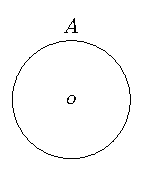
\includegraphics[]{figures/generic_set.pdf}
		\caption{The graphical representation of a generic set $A$ with generic element $o$.}
		\label{fig:generic_set}
	\end{figure}
\end{definition}

\begin{definition}[Membership]
	\label{def:membership}
	Given an object $o$ and a set $A$, the notation $o \in A$ denotes that $o$ is an element (or member) of $A$. If $o \notin A$, then $o$ is not an element of $A$.
\end{definition}

\begin{definition}[Cartesian Product]
	\label{def:cartesian_product}
	The Cartesian product of sets $A$ and $B$, denoted by $A \times B$, is defined as the set containing all ordered pairs $(a, b)$, where $a$ is in $A$ and $b$ is in $B$.
\end{definition}

\begin{example}
	Let $A = \{a_1, a_2\}$ and $B = \{b_1, b_2, b_3\}$ then
	\begin{equation}
		\begin{split}
			A\times B = \{&(a_1,b_1),(a_1,b_2),(a_1,b_3),\\
			&(a_2,b_1),(a_2,b_2),(a_2,b_3)\}.
		\end{split}
	\end{equation}
\end{example}

\begin{definition}[Subset]
	\label{def:subset}
	The set $A$ is called a subset\index{Subset} of the set $B$, denoted $A \subseteq B$, if every element of $A$ is also an element of $B$. Formally, 
	\begin{equation}
		A\subseteq B \quad \Longleftrightarrow \quad\forall x \in A \colon x\in B.
	\end{equation}
	By this definition, a set is always a subset of itself.
\end{definition}

\begin{definition}[Proper Subset]
	\label{def:proper_subset}
	The set $A$ is called a proper subset of the set $B$, denoted $A \subset B$, if $A \subseteq B$ and $A \neq B$. This means that $A$ is a subset of $B$ but $A$ is not equal to $B$; there is at least one element in $B$ that is not in $A$.
	\begin{figure}[H]
		\centering
		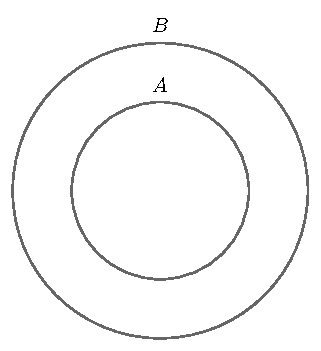
\includegraphics[]{figures/set_subset.pdf}
		\caption{The graphical representation of $A\subset B$.}
		\label{fig:set_subset}
	\end{figure}
\end{definition}

\newpage
\begin{example}
	$\twemoji{banana}$, $\twemoji{apple}$, and $\twemoji{eggplant}$ are members (elements) of the set $\{\twemoji{banana}, \twemoji{apple}, \twemoji{eggplant}\}$, but are not subsets of it; in turn, the subsets, such as $\{\twemoji{banana},\twemoji{apple}\}$, are not members of the set $\{\twemoji{banana}, \twemoji{apple}, \twemoji{eggplant}\}$.
\end{example}

\begin{example}
	Suppose $A = \{\twemoji{banana}, \twemoji{apple}, \twemoji{eggplant}\}$, then $\{\twemoji{banana}, \twemoji{apple}\}$ and $\{\twemoji{apple}\}$ are proper subsets of $A$, meaning $\{\twemoji{banana}, \twemoji{apple}\},\{\twemoji{apple}\}\subset  A$. $\{\twemoji{banana}, \twemoji{carrot}\}$, on the other hand, is not a subset of $A$, meaning $\{\twemoji{banana}, \twemoji{carrot}\}\not\subset  A$.
\end{example}

\begin{definition}[Empty Set]
	The empty set\index{Empty set}, denoted by $\emptyset$ or $\{\}$, is the set that contains no elements.
\end{definition}

\begin{definition}[Power Set]
	\label{def:power_set}
	The power set\index{Power set} of a set $A$, denoted by $2^A$, is defined as the set containing all possible subsets of $A$, including $A$ itself and the empty set.
\end{definition}

\begin{example}
	The power set of the set $A = \{a_1,a_2,a_3\}$ can be written
	\begin{equation}
		\begin{split}
			2^A = \{&\emptyset, \{a_1\}, \{a_2\}, \{a_3\}, \{a_1, a_2\},\\
			& \{a_1, a_3\}, \{a_2, a_3\}, A\}.
		\end{split}
	\end{equation}
\end{example}

\begin{definition}[Universal Set]
	\label{def:universal_set}
	The universal set\index{Universal set}, denoted by $\Omega$, is the set that contains all the objects or elements under consideration in a particular discussion or problem. It is the largest set in the context of a given study.
\end{definition}

\begin{definition}[Closure]
	\label{def:closure}
	The set $A$ is said to be closed under a certain operation if, for every pair of elements $x,y\in A$, the result of applying the operation to $x$ $y$ is also in $A$.
\end{definition}

\begin{definition}[Closure]
	A set $A$ is said to be \emph{closed under an operation} $\ast$ if, for all $x, y \in A$, the result of applying $\ast$ to $x$ and $y$ is also an element of $A$; that is,
	\begin{equation}
		x, y \in A \;\Rightarrow\; x \ast y \in A.
	\end{equation}
\end{definition}

\begin{example}
	Let $\mathcal{E} = \{ 2k \mid k \in \mathbb{Z} \}$ denote the set of even integers.
	Then $\mathcal{E}$ is closed under addition, since for any $x, y \in \mathcal{E}$,
	\begin{equation}
		x + y \in \mathcal{E}.
	\end{equation}
	In contrast, the set of odd integers $\mathbb{O} = \{ 2k + 1 \mid k \in \mathbb{Z} \}$ is not closed under addition, because $x + y$ is even when $x, y \in \mathbb{O}$.
\end{example}

\newpage
\begin{definition}[Union]
	The union of sets $A$ and $B$, denoted by $A \cup B$, is defined as the set containing all elements that are in $A$ or $B$ (or both). \figref{fig:set_union} provides a graphical representation of $A \cup B$.
	\begin{figure}[h]
		\centering
		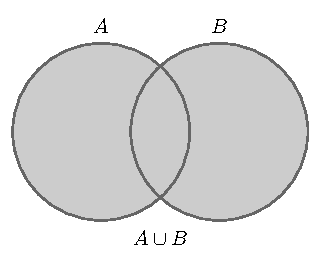
\includegraphics[]{figures/set_union.pdf}
		\caption{The graphical representation of $A\cup B$. Each circle represents the sets and the colored region represents the result of the binary operation.}
		\label{fig:set_union}
	\end{figure}
\end{definition}

\begin{definition}[Finite and Infinite Unions]
	For a collection of sets $\{A_i\}$, the union is denoted by $\bigcup_{i} A_i$ and is defined as the set containing all elements that are in at least one of the sets $A_i$.
\end{definition}

\begin{definition}[Intersection]
	The intersection of sets $A$ and $B$, denoted by $A \cap B$, is defined as the set containing all elements that are common to both $A$ and $B$. \figref{fig:set_intersection} provides a graphical representation of $A \cap B$.
	\begin{figure}[H]
		\centering
		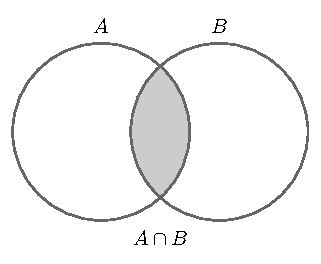
\includegraphics[]{figures/set_intersection.pdf}
		\caption{The graphical representation of $A\cap B$. Each circle represents the sets and the colored region represents the result of the binary operation.}
		\label{fig:set_intersection}
	\end{figure}
\end{definition}

\begin{definition}[Finite and Infinite Intersections]
	For a collection of sets $\{A_i\}$, the intersection is denoted by $\bigcap_{i} A_i$ and is defined as the set containing all elements that are common to all sets $A_i$.
\end{definition}

\begin{definition}[Disjoint]
	Two sets $A$ and $B$ are said to be disjoint if their intersection is the empty set, i.e., $A \cap B = \emptyset$. \figref{fig:set_disjoint} provides a graphical representation of $A \cap B=\emptyset$.
	\begin{figure}[H]
		\centering
		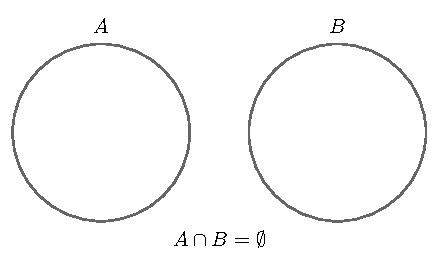
\includegraphics[]{figures/set_disjoint.pdf}
		\caption{The graphical representation of $A\cap B= \emptyset$. Each circle represents the sets and the colored region represents the result of the binary operation.}
		\label{fig:set_disjoint}
	\end{figure}
\end{definition}


\begin{definition}[Complementation]
	\label{def:complementation}
	The complement of set $A$, denoted by $A^c$, is defined as the set containing all elements in the universal set $\Omega$ that are not in $A$. \figref{fig:set_complementation} provides a graphical representation of $(A \cap B)^c$.
	\begin{figure}[H]
		\centering
		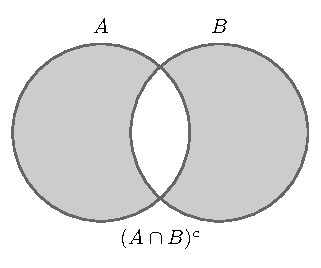
\includegraphics[]{figures/set_complementary.pdf}
		\caption{The graphical representation of $(A \cap B)^c$. Each circle represents the sets and the colored region represents the result of the binary operation.}
		\label{fig:set_complementation}
	\end{figure}
\end{definition}

\begin{definition}[Difference]
	The difference between sets $A$ and $B$, denoted by $A \setminus B = A\cap B^c$, is defined as the set containing all elements in $A$ that are not in $B$. \figref{fig:set_minus} provides a graphical representation of $A\setminus B$ and $B\setminus A$.
	\begin{figure}[H]
		\centering
		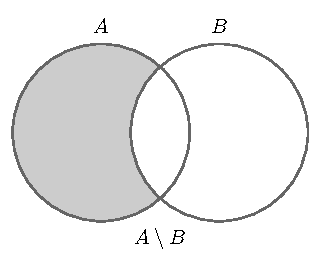
\includegraphics[]{figures/set_minus.pdf}
		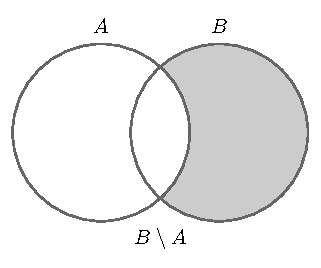
\includegraphics[]{figures/set_minus2.pdf}
		\caption{The graphical representation of $A\setminus B$ (left) and $B\setminus A$ (right). Each circle represents the sets and the colored region represents the result of the binary operation.}
		\label{fig:set_minus}
	\end{figure}
\end{definition}

\begin{definition}[Symmetric Difference]
	The symmetric difference of sets $A$ and $B$, denoted by $A \Delta B$, is defined as the set containing all elements that are in either $A$ or $B$ but not in both, meaning $A \Delta B = (A \cap B)^c$. \figref{fig:set_complementation} shows the symmetric difference between sets $A$ and $B$.
\end{definition}



\begin{definition}[Partition]
	\label{def:partition}
	A collection of non-empty subsets $\{A_i\}$ of a set $A$ is called a partition of $A$ if the following conditions are satisfied:
	\begin{enumerate}
		\item The subsets $A_i$ are pairwise disjoint, i.e., $A_i \cap A_j = \emptyset$ for all \(i \neq j\).
		\item The union of all subsets $A_i$ is equal to the set $A$, i.e., $\bigcup_{i \in I} A_i = A$.
	\end{enumerate}
	
	A graphical representation of the set $A=\{A_1,A_2,A_3\}$, where $A_j$ are partitions, is shown in \figref{fig:set_partition}.
	\begin{figure}[h]
		\centering
		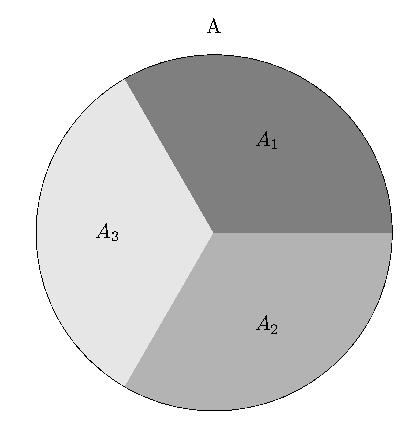
\includegraphics[]{figures/set_partition.pdf}
		\caption{A graphical representation of $A = \{A_1, A_2, A_3\}$, where the $A_j$ are the disjoint subsets forming a partition of $A$.}
		\label{fig:set_partition}
	\end{figure}
\end{definition}
